\documentclass[11pt,a4paper,]{article}
\usepackage{lmodern}

\usepackage{amssymb,amsmath}
\usepackage{ifxetex,ifluatex}
\usepackage{fixltx2e} % provides \textsubscript
\ifnum 0\ifxetex 1\fi\ifluatex 1\fi=0 % if pdftex
  \usepackage[T1]{fontenc}
  \usepackage[utf8]{inputenc}
\else % if luatex or xelatex
  \usepackage{unicode-math}
  \defaultfontfeatures{Ligatures=TeX,Scale=MatchLowercase}
\fi
% use upquote if available, for straight quotes in verbatim environments
\IfFileExists{upquote.sty}{\usepackage{upquote}}{}
% use microtype if available
\IfFileExists{microtype.sty}{%
\usepackage[]{microtype}
\UseMicrotypeSet[protrusion]{basicmath} % disable protrusion for tt fonts
}{}
\PassOptionsToPackage{hyphens}{url} % url is loaded by hyperref
\usepackage[unicode=true]{hyperref}
\hypersetup{
            pdftitle={ETC5513 Assignment 4: IMDB Data Analysis},
            pdfborder={0 0 0},
            breaklinks=true}
\urlstyle{same}  % don't use monospace font for urls
\usepackage{geometry}
\geometry{a4paper, centering, text={16cm,24cm}}
\usepackage[style=authoryear-comp,]{biblatex}
\addbibresource{references.bib}
\usepackage{longtable,booktabs}
% Fix footnotes in tables (requires footnote package)
\IfFileExists{footnote.sty}{\usepackage{footnote}\makesavenoteenv{long table}}{}
\usepackage{graphicx,grffile}
\makeatletter
\def\maxwidth{\ifdim\Gin@nat@width>\linewidth\linewidth\else\Gin@nat@width\fi}
\def\maxheight{\ifdim\Gin@nat@height>\textheight\textheight\else\Gin@nat@height\fi}
\makeatother
% Scale images if necessary, so that they will not overflow the page
% margins by default, and it is still possible to overwrite the defaults
% using explicit options in \includegraphics[width, height, ...]{}
\setkeys{Gin}{width=\maxwidth,height=\maxheight,keepaspectratio}
\IfFileExists{parskip.sty}{%
\usepackage{parskip}
}{% else
\setlength{\parindent}{0pt}
\setlength{\parskip}{6pt plus 2pt minus 1pt}
}
\setlength{\emergencystretch}{3em}  % prevent overfull lines
\providecommand{\tightlist}{%
  \setlength{\itemsep}{0pt}\setlength{\parskip}{0pt}}
\setcounter{secnumdepth}{5}

% set default figure placement to htbp
\makeatletter
\def\fps@figure{htbp}
\makeatother


\title{ETC5513 Assignment 4: IMDB Data Analysis}

%% MONASH STUFF

%% CAPTIONS
\RequirePackage{caption}
\DeclareCaptionStyle{italic}[justification=centering]
 {labelfont={bf},textfont={it},labelsep=colon}
\captionsetup[figure]{style=italic,format=hang,singlelinecheck=true}
\captionsetup[table]{style=italic,format=hang,singlelinecheck=true}


%% FONT
\RequirePackage{bera}
\RequirePackage[charter,expert,sfscaled]{mathdesign}
\RequirePackage{fontawesome}

%% HEADERS AND FOOTERS
\RequirePackage{fancyhdr}
\pagestyle{fancy}
\rfoot{\Large\sffamily\raisebox{-0.1cm}{\textbf{\thepage}}}
\makeatletter
\lhead{\textsf{\expandafter{\@title}}}
\makeatother
\rhead{}
\cfoot{}
\setlength{\headheight}{15pt}
\renewcommand{\headrulewidth}{0.4pt}
\renewcommand{\footrulewidth}{0.4pt}
\fancypagestyle{plain}{%
\fancyhf{} % clear all header and footer fields
\fancyfoot[C]{\sffamily\thepage} % except the center
\renewcommand{\headrulewidth}{0pt}
\renewcommand{\footrulewidth}{0pt}}

%% MATHS
\RequirePackage{bm,amsmath}
\allowdisplaybreaks

%% GRAPHICS
\RequirePackage{graphicx}
\setcounter{topnumber}{2}
\setcounter{bottomnumber}{2}
\setcounter{totalnumber}{4}
\renewcommand{\topfraction}{0.85}
\renewcommand{\bottomfraction}{0.85}
\renewcommand{\textfraction}{0.15}
\renewcommand{\floatpagefraction}{0.8}


%\RequirePackage[section]{placeins}

%% SECTION TITLES


%% SECTION TITLES
\RequirePackage[compact,sf,bf]{titlesec}
\titleformat*{\section}{\Large\sf\bfseries\color[rgb]{0.7,0,0}}
\titleformat*{\subsection}{\large\sf\bfseries\color[rgb]{0.7,0,0}}
\titleformat*{\subsubsection}{\sf\bfseries\color[rgb]{0.7,0,0}}
\titlespacing{\section}{0pt}{2ex}{.5ex}
\titlespacing{\subsection}{0pt}{1.5ex}{0ex}
\titlespacing{\subsubsection}{0pt}{.5ex}{0ex}


%% TITLE PAGE
\def\Date{\number\day}
\def\Month{\ifcase\month\or
 January\or February\or March\or April\or May\or June\or
 July\or August\or September\or October\or November\or December\fi}
\def\Year{\number\year}

%% LINE AND PAGE BREAKING
\sloppy
\clubpenalty = 10000
\widowpenalty = 10000
\brokenpenalty = 10000
\RequirePackage{microtype}

%% PARAGRAPH BREAKS
\setlength{\parskip}{1.4ex}
\setlength{\parindent}{0em}

%% HYPERLINKS
\RequirePackage{xcolor} % Needed for links
\definecolor{darkblue}{rgb}{0,0,.6}
\RequirePackage{url}

\makeatletter
\@ifpackageloaded{hyperref}{}{\RequirePackage{hyperref}}
\makeatother
\hypersetup{
     citecolor=0 0 0,
     breaklinks=true,
     bookmarksopen=true,
     bookmarksnumbered=true,
     linkcolor=darkblue,
     urlcolor=blue,
     citecolor=darkblue,
     colorlinks=true}

\usepackage[showonlyrefs]{mathtools}
\usepackage[no-weekday]{eukdate}

%% BIBLIOGRAPHY

\makeatletter
\@ifpackageloaded{biblatex}{}{\usepackage[style=authoryear-comp, backend=biber, natbib=true]{biblatex}}
\makeatother
\ExecuteBibliographyOptions{bibencoding=utf8,minnames=1,maxnames=3, maxbibnames=99,dashed=false,terseinits=true,giveninits=true,uniquename=false,uniquelist=false,doi=false, isbn=false,url=true,sortcites=false}

\DeclareFieldFormat{url}{\texttt{\url{#1}}}
\DeclareFieldFormat[article]{pages}{#1}
\DeclareFieldFormat[inproceedings]{pages}{\lowercase{pp.}#1}
\DeclareFieldFormat[incollection]{pages}{\lowercase{pp.}#1}
\DeclareFieldFormat[article]{volume}{\mkbibbold{#1}}
\DeclareFieldFormat[article]{number}{\mkbibparens{#1}}
\DeclareFieldFormat[article]{title}{\MakeCapital{#1}}
\DeclareFieldFormat[article]{url}{}
%\DeclareFieldFormat[book]{url}{}
%\DeclareFieldFormat[inbook]{url}{}
%\DeclareFieldFormat[incollection]{url}{}
%\DeclareFieldFormat[inproceedings]{url}{}
\DeclareFieldFormat[inproceedings]{title}{#1}
\DeclareFieldFormat{shorthandwidth}{#1}
%\DeclareFieldFormat{extrayear}{}
% No dot before number of articles
\usepackage{xpatch}
\xpatchbibmacro{volume+number+eid}{\setunit*{\adddot}}{}{}{}
% Remove In: for an article.
\renewbibmacro{in:}{%
  \ifentrytype{article}{}{%
  \printtext{\bibstring{in}\intitlepunct}}}

\AtEveryBibitem{\clearfield{month}}
\AtEveryCitekey{\clearfield{month}}

\makeatletter
\DeclareDelimFormat[cbx@textcite]{nameyeardelim}{\addspace}
\makeatother

\author{{\sf\Large\textbf{Mr Will Nguyen}\\\sf\large Master of Actuarial Science\\[0.5cm]}{\sf\Large\textbf{Ms Wang Xue}\\\sf\large Master of Business\\[0.5cm]}{\sf\Large\textbf{Mr Rahul Bharadwaj Mysore Venkatesh}\\\sf\large Master of Business Analytics\\[0.5cm]}{\sf\Large\textbf{Mr Aryan Jain}\\\sf\large Master of Business Analytics\\[0.5cm]}

\date{\sf\Date~\Month~\Year}
\makeatletter
\lfoot{\sf Nguyen, Xue, Mysore Venkatesh, Jain: \@date}
\makeatother


%%%% PAGE STYLE FOR FRONT PAGE OF REPORTS

\makeatletter
\def\organization#1{\gdef\@organization{#1}}
\def\telephone#1{\gdef\@telephone{#1}}
\def\email#1{\gdef\@email{#1}}
\makeatother
  \organization{Monash University}

  \def\name{Department of\newline Econometrics \&\newline Business Statistics}

  \telephone{(03) 9905 2478}

  \email{BusEco-Econometrics@monash.edu}

\def\webaddress{\url{http://buseco.monash.edu/ebs/consulting/}}
\def\abn{12 377 614 012}
\def\logo{
\includegraphics[width=6cm]{MBSportrait}}
\def\extraspace{\vspace*{1.6cm}}
\makeatletter
\def\contactdetails{\faicon{phone} & \@telephone \\
                    \faicon{envelope} & \@email}
\makeatother

%%%% FRONT PAGE OF REPORTS

\def\reporttype{Report for}

\long\def\front#1#2#3{
\newpage
\begin{singlespacing}
\thispagestyle{empty}
\vspace*{-1.4cm}
\hspace*{-1.4cm}
\hbox to 16cm{
  \hbox to 6.5cm{\vbox to 14cm{\vbox to 25cm{
    \logo
    \vfill
    \parbox{6.3cm}{\raggedright
      \sf\color[rgb]{0.00,0.00,0.70}
      {\large\textbf{\name}}\par
      \vspace{.7cm}
      \tabcolsep=0.12cm\sf\small
      \begin{tabular}{@{}ll@{}}\contactdetails
      \end{tabular}
      \vspace*{0.3cm}\par
      ABN: \abn\par
    }
  }\vss}\hss}
  \hspace*{0.2cm}
  \hbox to 1cm{\vbox to 14cm{\rule{1pt}{26.8cm}\vss}\hss\hfill}
  \hbox to 10cm{\vbox to 14cm{\vbox to 25cm{
      \vspace*{3cm}\sf\raggedright
      \parbox{11cm}{\sf\raggedright\baselineskip=1.2cm
         \fontsize{24.88}{30}\color[rgb]{0.70,0.00,0.00}\sf\textbf{#1}}
      \par
      \vfill
      \large
      \vbox{\parskip=0.8cm #2}\par
      \vspace*{2cm}\par
      \reporttype\\[0.3cm]
      \hbox{#3}%\\[2cm]\
      \vspace*{1cm}
      {\large\sf\textbf{\Date~\Month~\Year}}
   }\vss}
  }}
\end{singlespacing}
\newpage
}

\makeatletter
\def\titlepage{\front{\expandafter{\@title}}{\@author}{\@organization}}
\makeatother

\usepackage{setspace}
\setstretch{1.5}

\usepackage{booktabs}
\usepackage{longtable}
\usepackage{array}
\usepackage{multirow}
\usepackage{wrapfig}
\usepackage{float}
\usepackage{colortbl}
\usepackage{pdflscape}
\usepackage{tabu}
\usepackage{threeparttable}
\usepackage{threeparttablex}
\usepackage[normalem]{ulem}
\usepackage{makecell}
\usepackage{xcolor}


\begin{document}
\titlepage

\begin{verbatim}
## Warning: package 'tidyverse' was built under R version 4.0.5
\end{verbatim}

\begin{verbatim}
## Warning: package 'ggplot2' was built under R version 4.0.5
\end{verbatim}

\begin{verbatim}
## Warning: package 'tibble' was built under R version 4.0.5
\end{verbatim}

\begin{verbatim}
## Warning: package 'tidyr' was built under R version 4.0.5
\end{verbatim}

\begin{verbatim}
## Warning: package 'readr' was built under R version 4.0.5
\end{verbatim}

\begin{verbatim}
## Warning: package 'dplyr' was built under R version 4.0.5
\end{verbatim}

\begin{verbatim}
## Warning: package 'forcats' was built under R version 4.0.5
\end{verbatim}

\begin{verbatim}
## Warning: package 'kableExtra' was built under R version 4.0.5
\end{verbatim}

\begin{verbatim}
## Warning: package 'bookdown' was built under R version 4.0.5
\end{verbatim}

\begin{verbatim}
## Warning: package 'treemap' was built under R version 4.0.5
\end{verbatim}

\begin{verbatim}
## Warning: package 'viridis' was built under R version 4.0.5
\end{verbatim}

\begin{verbatim}
## Warning: package 'viridisLite' was built under R version 4.0.5
\end{verbatim}

\hypertarget{introduction}{%
\section{Introduction}\label{introduction}}

Due to the effects of Covid-19, there has been a significant increase in demand for in-home entertainment. One particular form of this entertainment that continues to thrive due to streaming services such as Netflix and Stan is watching movies. This report will be analysing a large dataset from the popular reviews website, IMDb. It will attempt to answer questions such as what periods experienced a significantly higher quality of movies and which streaming services offer the greatest variety of movies.

\begin{verbatim}
## Rows: 81,273
## Columns: 22
## $ imdb_title_id         <chr> "tt0000574", "tt0001892", "tt0002101", "tt000213~
## $ title                 <chr> "The Story of the Kelly Gang", "Den sorte drøm"~
## $ original_title        <chr> "The Story of the Kelly Gang", "Den sorte drøm"~
## $ year                  <int> 1906, 1911, 1912, 1911, 1912, 1919, 1913, 1912, ~
## $ date_published        <chr> "1906-12-26", "1911-08-19", "1912-11-13", "1911-~
## $ genre                 <chr> "Biography, Crime, Drama", "Drama", "Drama, Hist~
## $ duration              <int> 70, 53, 100, 68, 60, 85, 120, 120, 55, 121, 54, ~
## $ country               <chr> "Australia", "Germany, Denmark", "USA", "Italy",~
## $ language              <chr> "", "", "English", "Italian", "English", "German~
## $ director              <chr> "Charles Tait", "Urban Gad", "Charles L. Gaskill~
## $ writer                <chr> "Charles Tait", "Urban Gad, Gebhard Schätzler-P~
## $ production_company    <chr> "J. and N. Tait", "Fotorama", "Helen Gardner Pic~
## $ actors                <chr> "Elizabeth Tait, John Tait, Norman Campbell, Bel~
## $ description           <chr> "True story of notorious Australian outlaw Ned K~
## $ avg_vote              <dbl> 6.1, 5.9, 5.2, 7.0, 5.7, 6.8, 6.2, 6.7, 5.5, 6.7~
## $ votes                 <int> 537, 171, 420, 2019, 438, 709, 241, 187, 211, 31~
## $ budget                <chr> "$ 2250", "", "$ 45000", "", "", "", "ITL 45000"~
## $ usa_gross_income      <chr> "", "", "", "", "", "", "", "", "", "", "", "", ~
## $ worlwide_gross_income <chr> "", "", "", "", "", "", "", "", "", "", "", "", ~
## $ metascore             <dbl> NA, NA, NA, NA, NA, NA, NA, NA, NA, NA, NA, NA, ~
## $ reviews_from_users    <dbl> 7, 4, 24, 28, 12, 11, 6, 3, 7, 9, 9, 16, 8, 2, 6~
## $ reviews_from_critics  <dbl> 7, 2, 3, 14, 5, 9, 4, 1, 1, 9, 29, 7, 22, 2, 17,~
\end{verbatim}

\hypertarget{williams-section}{%
\section{William's Section}\label{williams-section}}

According to IMDb, metascore is a single number that represents the overall critical opinion about a movie. Its legitimacy is derived from applying a weighted average to the reviews of the world's most respected critics. That said, metascore is still an extremely vague concept - particularly when it comes to the threshold of what metascore can be considered good.

\begin{table}

\caption{\label{tab:metascoretable}Metascore summary}
\centering
\begin{tabular}[t]{l|l}
\hline
  &   metascore\\
\hline
 & Min.   :  1.00\\
\hline
 & 1st Qu.: 43.00\\
\hline
 & Median : 56.00\\
\hline
 & Mean   : 55.76\\
\hline
 & 3rd Qu.: 69.00\\
\hline
 & Max.   :100.00\\
\hline
 & NA's   :68551\\
\hline
\end{tabular}
\end{table}

Therefore, it is important to first consider the distribution of metascore within the data set. This is summarised by Table \ref{tab:metascoretable}. The most noteworthy features are that the median and mean are very close at 56 and 55.76 respectively and nearly 70,000 movies have not been assigned a metascore. Consequently, any analysis related to the metascore variable must be treated with caution as less than 20\% of the movies are represented.

\begin{figure}
\centering
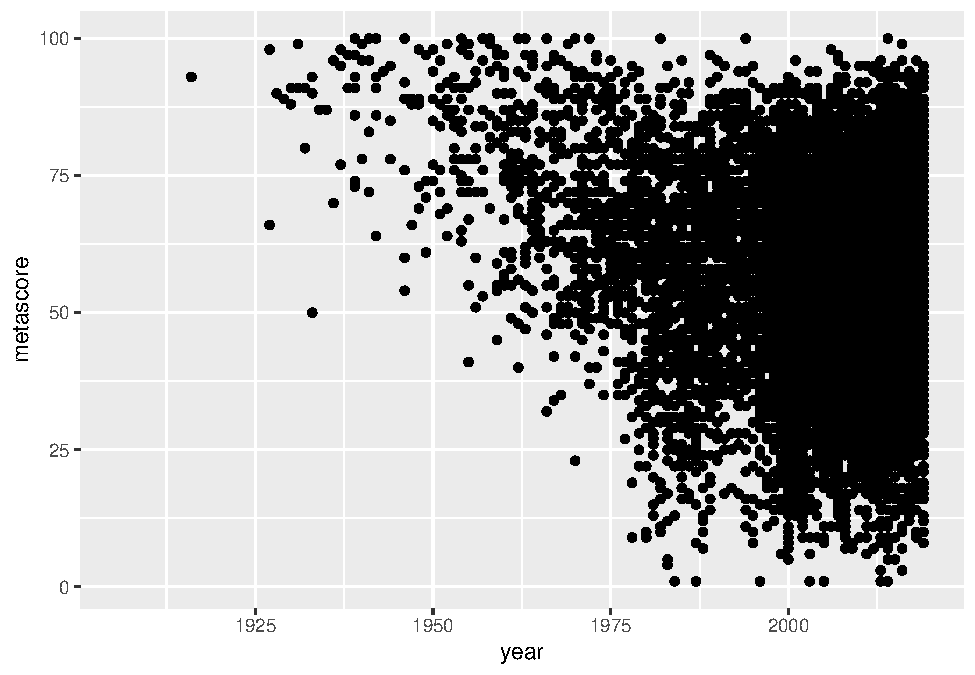
\includegraphics{Report_files/figure-latex/metascorescatterplot-1.pdf}
\caption{\label{fig:metascorescatterplot}metascore vs time}
\end{figure}

As expected, the scatter plot depicted in Figure \ref{fig:metascorescatterplot} is not particularly informative and potentially misleading. Although the spread is increasing, one can still identify a negative correlation which suggests that the quality of movies has degraded over time. However, it is important to recognise that this dataset was taken from IMDb which means that sampling was far from random. IMDb has much more incentive to review recently released movies. Hence, when older movies are reviewed, it is likely because it is still immensely popular (i.e.~a `classic').

\begin{table}

\caption{\label{tab:toptwentytable}The top 20 movies arranged by metascore}
\centering
\begin{tabular}[t]{l|r|r}
\hline
title & year & metascore\\
\hline
The Wizard of Oz & 1939 & 100\\
\hline
Citizen Kane & 1941 & 100\\
\hline
Casablanca & 1942 & 100\\
\hline
Notorious & 1946 & 100\\
\hline
Viaggio in Italia & 1954 & 100\\
\hline
Rear Window & 1954 & 100\\
\hline
Sweet Smell of Success & 1957 & 100\\
\hline
Vertigo & 1958 & 100\\
\hline
Lawrence of Arabia & 1962 & 100\\
\hline
Il gattopardo & 1963 & 100\\
\hline
Au hasard Balthazar & 1966 & 100\\
\hline
Il conformista & 1970 & 100\\
\hline
The Godfather & 1972 & 100\\
\hline
Fanny och Alexander & 1982 & 100\\
\hline
Trois couleurs: Rouge & 1994 & 100\\
\hline
Boyhood & 2014 & 100\\
\hline
City Lights & 1931 & 99\\
\hline
Pinocchio & 1940 & 99\\
\hline
Singin' in the Rain & 1952 & 99\\
\hline
The Night of the Hunter & 1955 & 99\\
\hline
\end{tabular}
\end{table}

\begin{figure}
\centering
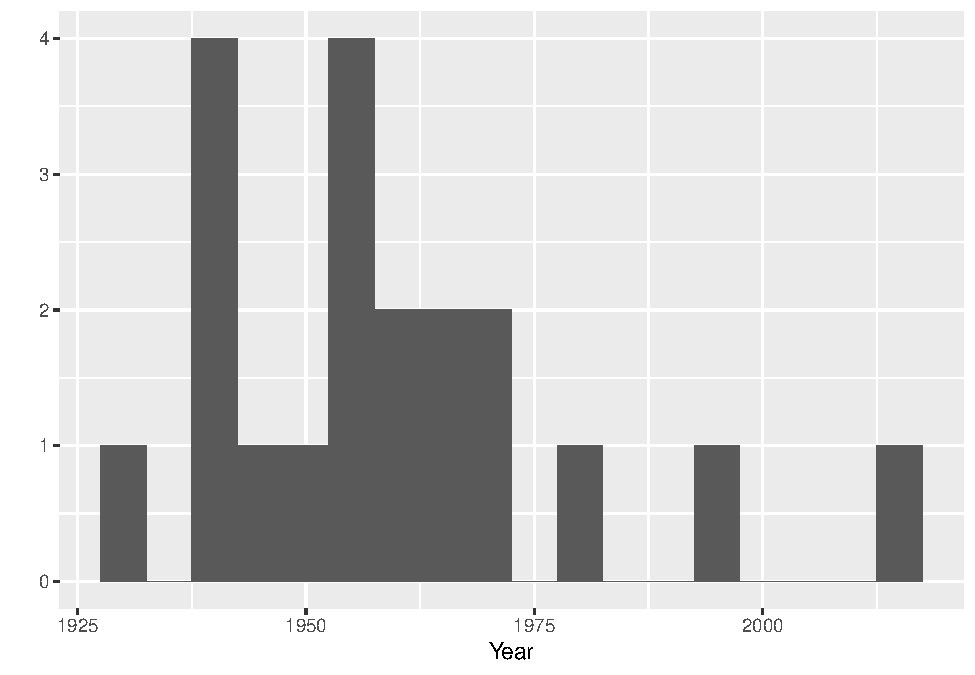
\includegraphics{Report_files/figure-latex/toptwentyhistogram-1.pdf}
\caption{\label{fig:toptwentyhistogram}Time distribution of top twenty movies}
\end{figure}

The aforementioned `classics bias' is further confirmed by both Table \ref{tab:toptwentytable} and Figure \ref{fig:toptwentyhistogram}. This list is dominated by the most famous movies from the 1900's such as The Wizard of Oz, Citizen Kane and The Godfather which were all assigned perfect metascores. Moreover, seventeen of the twenty listed movies were released before 1975 and only one was released after 2000.

Assuming that metascore is a reliable representation of a movie's quality, it is easy to see why arguments have been made that movies produced in recent times are not as good. Contrarily, a counterargument can be made that there were just as many bad movies made during previous generations that have been forgotten or overshadowed by the classics. Due to the clear bias within this dataset, it is still unclear which argument is stronger.

\hypertarget{xue-wangs-section}{%
\section{Xue Wang's Section}\label{xue-wangs-section}}

\hypertarget{language}{%
\subsection{Language}\label{language}}

\hypertarget{the-proportion-of-top-100-movie-language}{%
\subsubsection{The proportion of top 100 movie language}\label{the-proportion-of-top-100-movie-language}}

\begin{figure}
\centering
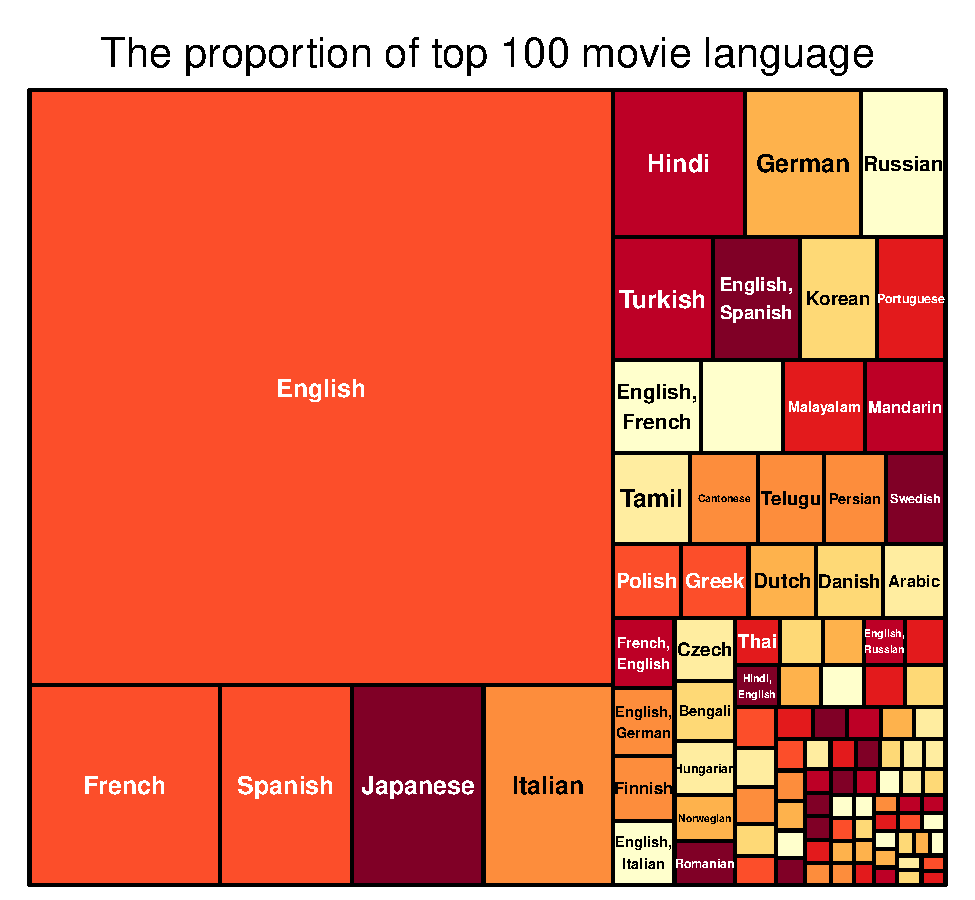
\includegraphics{Report_files/figure-latex/language-1.pdf}
\caption{\label{fig:language}The proportion of top 100 movie language}
\end{figure}

The figure \ref{fig:language} shows the proportion of the number top 100 languages. It can clearly be seen that the English movies account for almost half of all movies. French, Spanish, Japanese, Italian almost have the same proportion with the number of above 2500. It is very clear to see the situation about the distribution.

\hypertarget{number-of-top-9-languages-between-2009-and-2019}{%
\subsubsection{Number of top 9 languages between 2009 and 2019}\label{number-of-top-9-languages-between-2009-and-2019}}

\begin{figure}
\centering
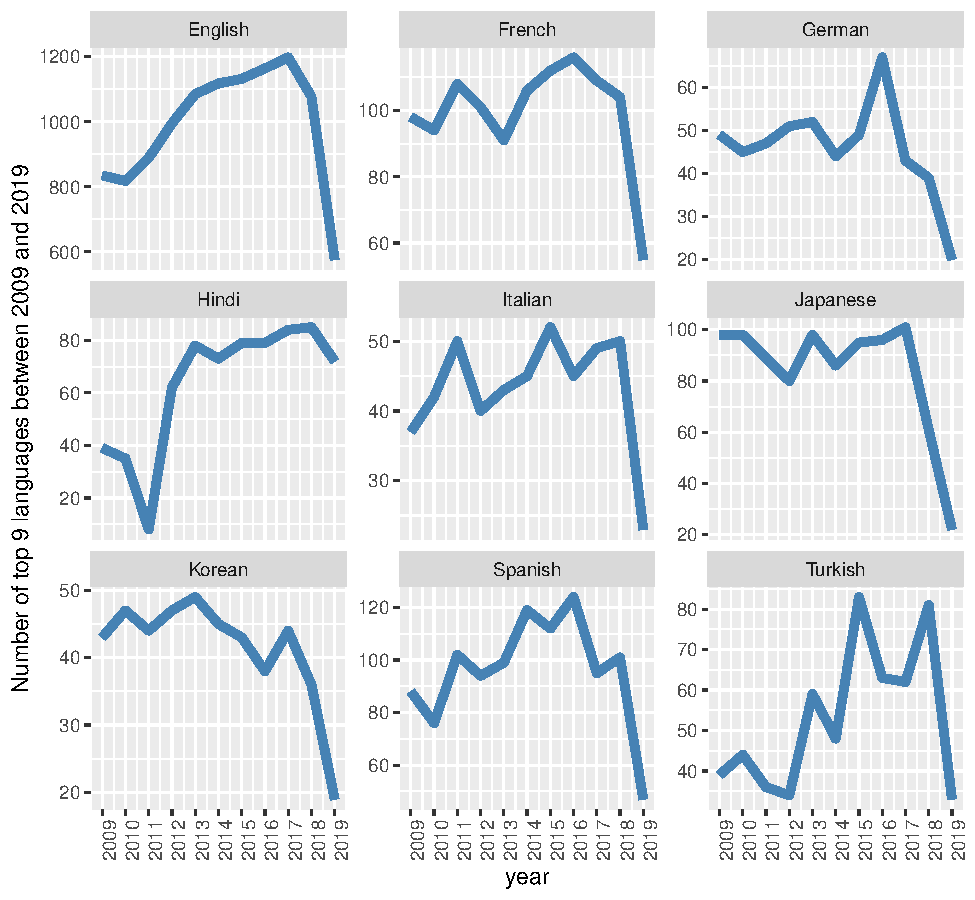
\includegraphics{Report_files/figure-latex/langyear-1.pdf}
\caption{\label{fig:langyear}Top 9 languages between 2009 and 2019}
\end{figure}

The figure \ref{fig:langyear} shows the number of different languages movies between 2009 and 2019. It can be clearly seen that the largest number of movie languages is English, it has an increasing trend between 2009 and 2017 and will drop to 600 in 2019. The number of Korean language movies have the minimum quantity within the 9 languages, it shows a decreasing trend during the ten years. The number of French,German, Japanese and Italian, they almost maintained the level from 2009 to 2017, and then sharply decreased to 2019.

\hypertarget{genres}{%
\subsection{Genres}\label{genres}}

\hypertarget{the-proportion-of-top-100-movie-genres}{%
\subsubsection{The proportion of top 100 movie genres}\label{the-proportion-of-top-100-movie-genres}}

\begin{figure}
\centering
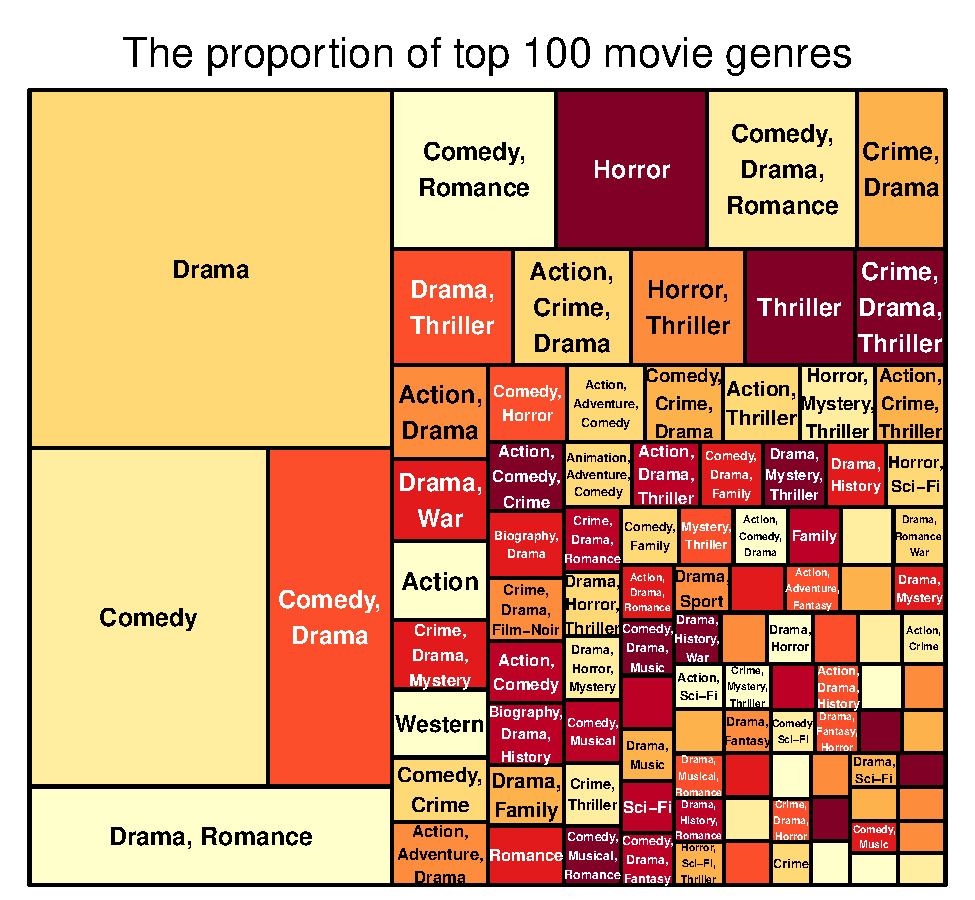
\includegraphics{Report_files/figure-latex/genres-1.pdf}
\caption{\label{fig:genres}The proportion of top 100 movie genres}
\end{figure}

The figure \ref{fig:genres} shows the proportion of top 100 movie genres, from the figure, we can see that the drama and comedy almost occupied 30\% of total movies, followed by the horror, comedy and romance, drama and romance, thriller.etc almost have the same proportion, this picture clearly shows the proportion of different movie genres.

\hypertarget{number-of-top-10-genres-of-movies-published-from-2009-to-2019}{%
\subsubsection{Number of top 10 genres of movies published from 2009 to 2019}\label{number-of-top-10-genres-of-movies-published-from-2009-to-2019}}

\begin{figure}
\centering
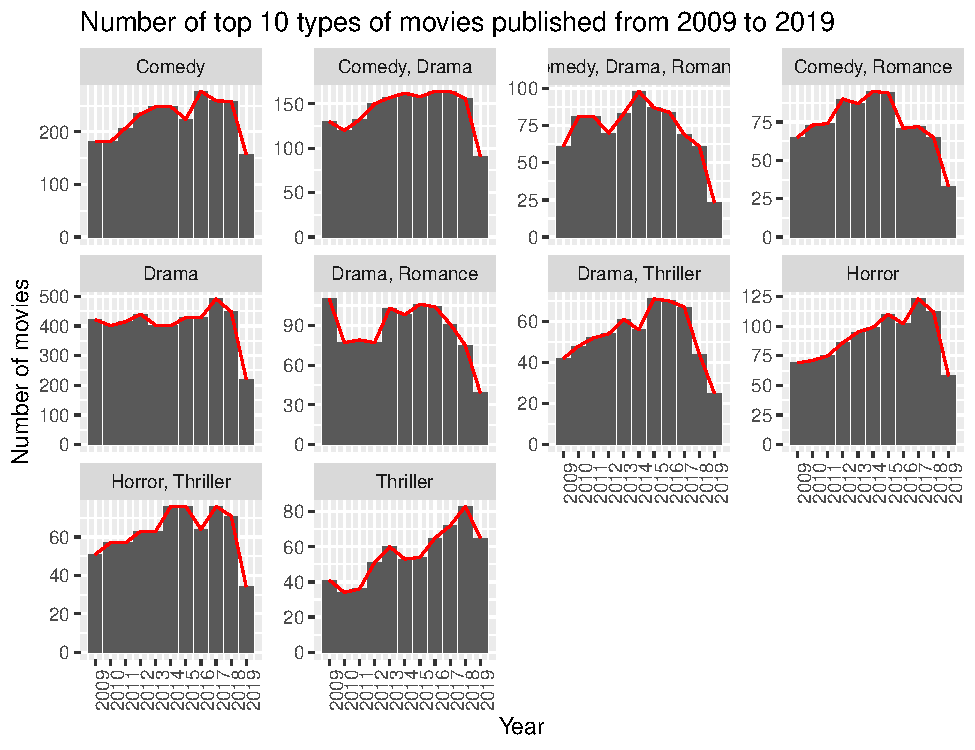
\includegraphics{Report_files/figure-latex/genresyear-1.pdf}
\caption{\label{fig:genresyear}Number of top 10 types of movies published from 2009 to 2019}
\end{figure}

The figure \ref{fig:genresyear} graph shows the change in the number of different movie genres in ten years, from this figure, it can be seen that,the number of dramas and comedies almost exceeds 100 every year, and dramas almost reach 500 every year. When it comes to the line chart, the number of almost all movie genres peaked in 2017 and then fell to 2019. This is because the movie industry returns to the content ontology and enters the transition period from quantity to quality.

\hypertarget{the-largest-number-of-movies-genres-in-each-country}{%
\subsubsection{The largest number of movies genres in each country}\label{the-largest-number-of-movies-genres-in-each-country}}

\begin{table}

\caption{\label{tab:maxgenres} The largest number of movies genres in each country}
\centering
\begin{tabular}[t]{llr}
\toprule
country & genre & n\\
\midrule
USA & Drama & 1252\\
India & Drama & 436\\
France & Drama & 334\\
Italy & Comedy & 295\\
Japan & Drama & 267\\
\addlinespace
Canada & Drama & 217\\
Germany & Drama & 215\\
UK & Drama & 171\\
Turkey & Comedy & 166\\
Spain & Drama & 163\\
\bottomrule
\end{tabular}
\end{table}

Table \ref{tab:maxgenres} show the largest number of movies genres in each country in the 21st century, according to this table, we can see the the largest number of movies in many countries is drama, According Table \ref{tab:pretdrame} , it shows the drama has the largest proportion with 58.84\%, However, the second place comedy only reached 8\%.

\begin{table}

\caption{\label{tab:pretdrame} The largest number of movies genres in each country}
\centering
\begin{tabular}[t]{lrrr}
\toprule
genre & total & total\_movies & prop\_genre\\
\midrule
Drama & 6534 & 11103 & 0.5884896\\
Comedy & 914 & 11103 & 0.0823201\\
Comedy, Drama & 290 & 11103 & 0.0261191\\
Drama, Romance & 239 & 11103 & 0.0215257\\
Comedy, Drama, Romance & 121 & 11103 & 0.0108980\\
\bottomrule
\end{tabular}
\end{table}

\newpage

\hypertarget{rahuls-section.}{%
\section{Rahul's Section.}\label{rahuls-section.}}

\hypertarget{movie-grosses-and-popularity-analysis}{%
\subsection{Movie Grosses and Popularity Analysis}\label{movie-grosses-and-popularity-analysis}}

\begin{itemize}
\item
  What is the Budget and USA Gross for Avenger and Spider-Man movie franchises?
\item
  What is the Number of user reviews and critic reviews for the same, implying their popularity?
\item
  What is the gross of the most popular movies of all-time?
\end{itemize}

Tidyverse (\textcite{tidyverse}) is used to clean the data and kableExtra (\textcite{kableExtra}) is used to display tables.

\begin{table}

\caption{\label{tab:GrossTable}Sample Gross Data Table}
\centering
\begin{tabular}[t]{lll}
\toprule
Title & Budget & USA\_Gross\\
\midrule
Das Cabinet des Dr. Caligari & \$ 18000 & \$ 8811\\
The Four Horsemen of the Apocalypse & \$ 800000 & \$ 9183673\\
Metropolis & DEM 6000000 & \$ 1236166\\
City Lights & \$ 1500000 & \$ 19181\\
Modern Times & \$ 1500000 & \$ 163577\\
\addlinespace
Snow White and the Seven Dwarfs & \$ 1499000 & \$ 184925486\\
Gone with the Wind & \$ 3977000 & \$ 200852579\\
Mr. Smith Goes to Washington & \$ 1900000 & \$ 144738\\
La règle du jeu & FRF 5500500 & \$ 273641\\
The Wizard of Oz & \$ 2777000 & \$ 24790250\\
\bottomrule
\end{tabular}
\end{table}

The table \ref{tab:GrossTable} shows a sample of the gross data used for the analysis. The main columns needed for Gross analysis are Title, Budget, and USA\_Gross.

\begin{table}

\caption{\label{tab:ReviewTable}Sample Review Data Table}
\centering
\begin{tabular}[t]{lrr}
\toprule
Title & User\_Reviews & Critic\_Reviews\\
\midrule
The Story of the Kelly Gang & 7 & 7\\
Den sorte drøm & 4 & 2\\
Cleopatra & 24 & 3\\
L'Inferno & 28 & 14\\
From the Manger to the Cross; or, Jesus of Nazareth & 12 & 5\\
\addlinespace
Madame DuBarry & 11 & 9\\
Quo Vadis? & 6 & 4\\
Independenta Romaniei & 3 & 1\\
Richard III & 7 & 1\\
Atlantis & 9 & 9\\
\bottomrule
\end{tabular}
\end{table}

The table \ref{tab:ReviewTable} shows a sample of the review data used for the analysis. The main columns needed for Gross analysis are Title, User\_Reviews, and Critic\_Reviews.

Using the table contents, we plot data for a particular movie franchise. The franchises selected for this anlysis are Avengers and Spider-Man. We display plots to analyse how much the franchise spent for the movie and how much it grossed. Also a plot for the user reviews and critic reviews are displayed to see which were the most popular among all the movies in the franchise. We also plot the same for all the movies in the dataset.

\begin{figure}[H]

{\centering 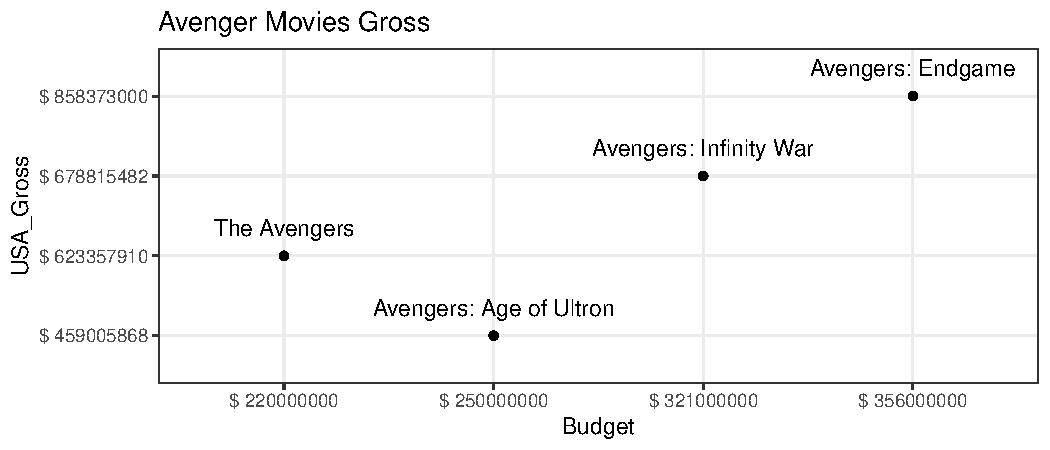
\includegraphics{Report_files/figure-latex/AvengersGross-1} 

}

\caption{Avengers Budget v/s Gross}\label{fig:AvengersGross}
\end{figure}

From the figure \ref{fig:AvengersGross}, it can be seen that all Avenger movies grossed more than the amount spent. Avengers: Age of Ultron grossed relatively lesser than the other movies. Endgame was the highest grossing Avenger movie.

\begin{figure}[H]

{\centering 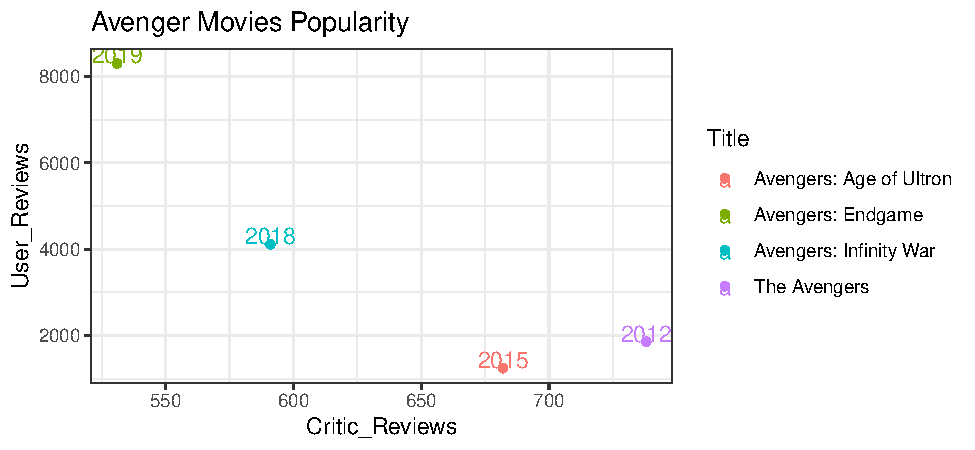
\includegraphics{Report_files/figure-latex/AvengersReview-1} 

}

\caption{Avengers Popularity}\label{fig:AvengersReview}
\end{figure}

The figure \ref{fig:AvengersReview} displays how many reviews was given by users and critics. This can be a measure of how much the movies were talked about. The year tags show the timeline. It is evident that the first avenger movie in 2012 attracted the attention of critics with a high number of critic reviews. As time passed by, the movies become more popular among users which shows an increse in the fanbase till 2019. The only exception to this is a dip in user reviews for Age of Ultron which justifies why it grossed lesser than other movies.

\begin{figure}[H]

{\centering 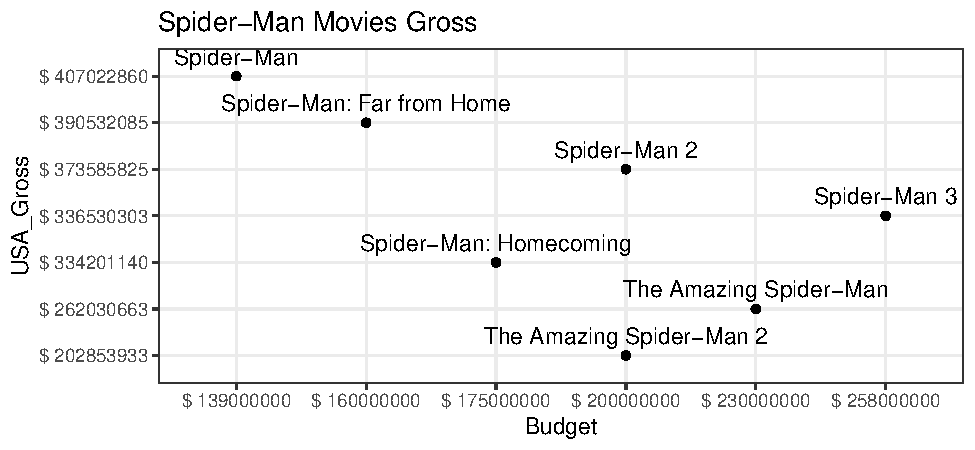
\includegraphics{Report_files/figure-latex/SpiderManPlot-1} 

}

\caption{Spider-Man Budget v/s Gross}\label{fig:SpiderManPlot}
\end{figure}

The figure \ref{fig:SpiderManPlot} shows the budget and gross of Spider-Man movies. Spider-Man grossed the highest and the sequels Spider-Man 2 and Spider-Man 3 grossed lesser showing a decline in the gross. The Amazing Spider-Man seems to have grossed better than its sequel The Amazing Spider-Man 2. These movies has grossed far less than the first 3 movies. The Homecoming and Far from Home movies seem to have made a great comeback in terms of its gross compared to the fourth and fifth movies. Far from Home has grossed more and spent less which makes it the second best Spider-Man movie after the first ever one in the franchise.

The figure \ref{fig:SpiderManReview} shows a graph for the number of reviews by critics and users over a period of time named by the years for each points. The first ever movie was most talked about by both fans and users in 2002. We see a dip in user reviews for 2004 and the movie in 2007 was a little better but the first ever was the best recieved. The fourth and fifth movies in 2012 and 2014 was talked about most by critics but never really kicked off among fans. This justifies its low grosses. The final sixth and seventh movies in 2017 and 2019 have made a great comeback after this dip and the latest one during 2019 has managed to almost equal the fanbase like it was when the franchise started.

\begin{figure}[H]

{\centering 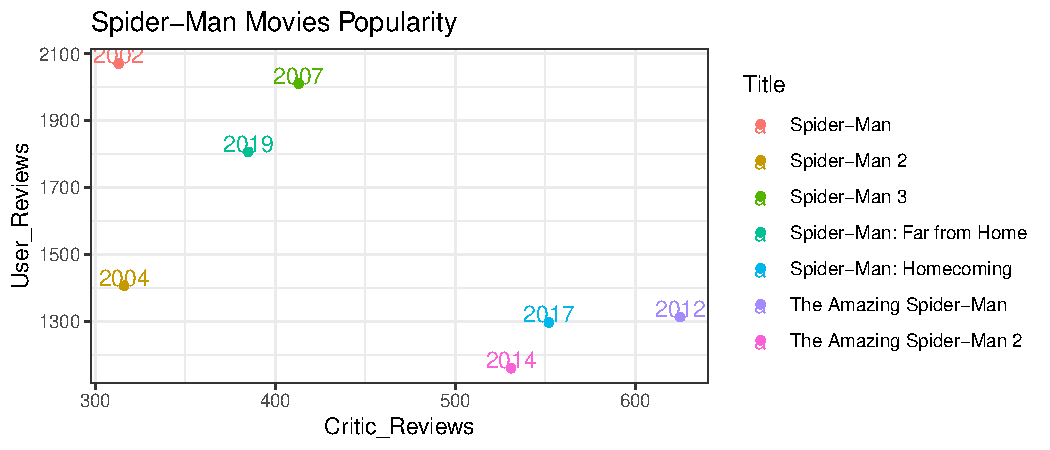
\includegraphics{Report_files/figure-latex/SpiderManReview-1} 

}

\caption{Spider-Man Popularity}\label{fig:SpiderManReview}
\end{figure}

\begin{figure}[H]

{\centering 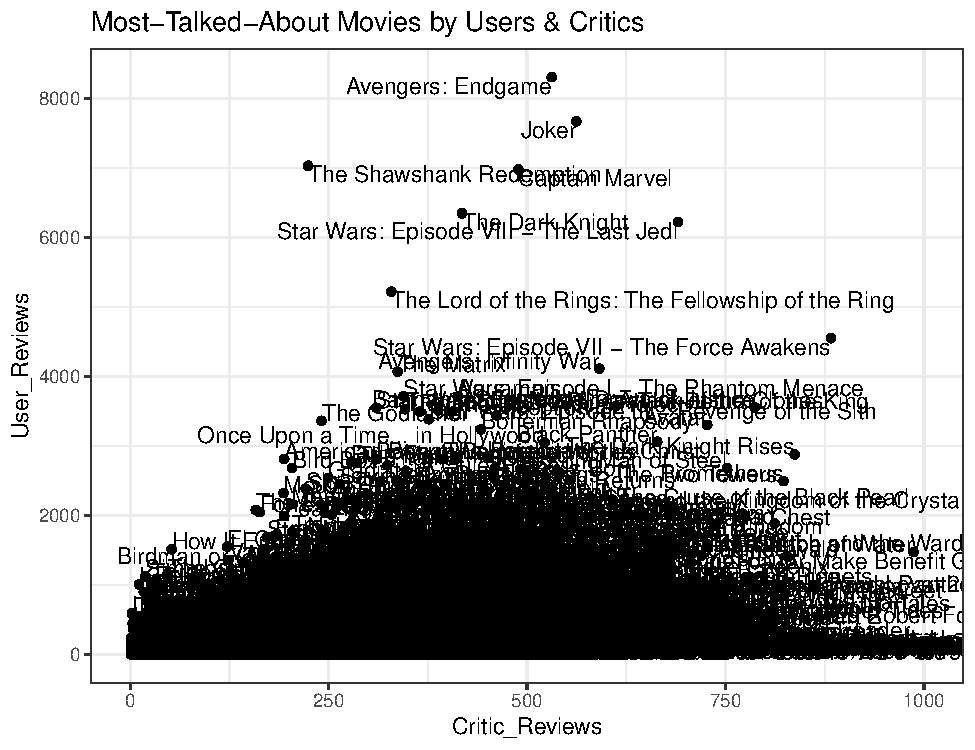
\includegraphics{Report_files/figure-latex/AllReviewsPlot-1} 

}

\caption{All-time Popularity}\label{fig:AllReviewsPlot}
\end{figure}

The figure \ref{fig:AllReviewsPlot} looks shabby when you first look at it but it has some insights that can be drawn from it. The black cluster at the left bottom are the movies that have a low number of reviews by both users and critics. These are the least popular movies. The outliers are clearly visible in this plot with Endgame being the most popular among fans around the globe. This plot is used to pick the most popular movies to be used to compare the budget and gross. It is not necessary for a movie to be good, to be most talked about. So the next plot serves as a verification to confirm if the movie was talked about because it was good, or bad.

\begin{figure}[H]

{\centering 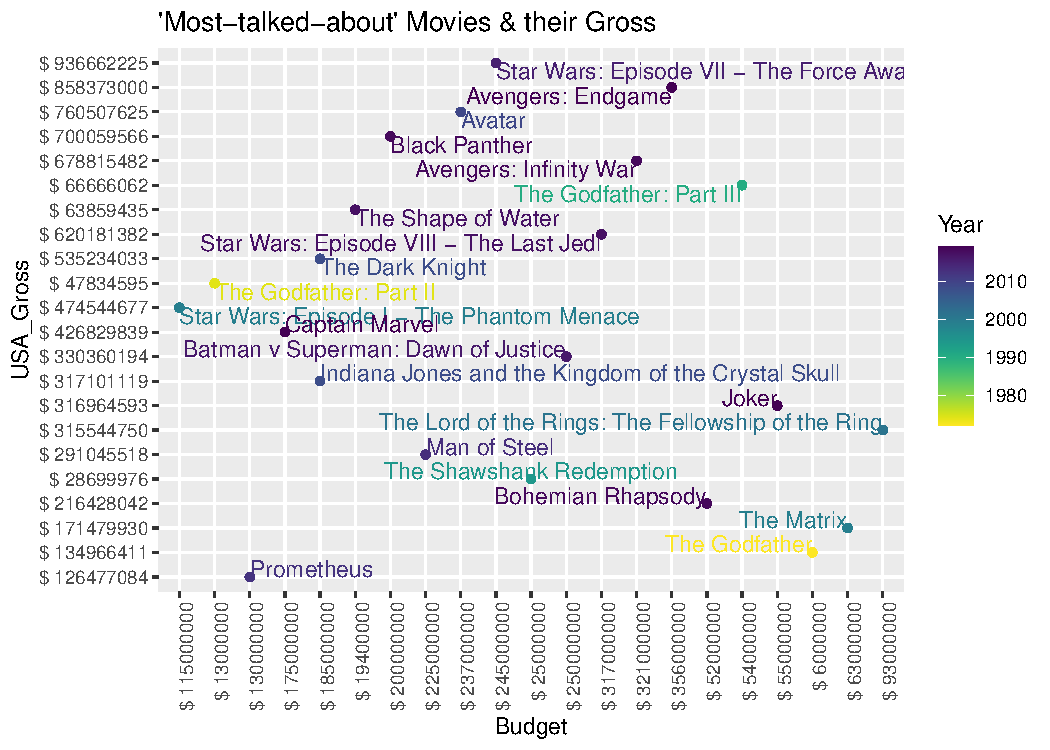
\includegraphics{Report_files/figure-latex/AllGrossPlot-1} 

}

\caption{Some all-time Popular Movies and their Gross}\label{fig:AllGrossPlot}
\end{figure}

The figure \ref{fig:AllGrossPlot} shows the budget and gross of the most popular movies from over a century. We can compare the production cost, which is the budget, and the gross to ensure that it was most talked about because it was good. This plot also has information about the decade it was released in. This was to ensure there was no bias between the movies since currency value is always changing. The values are discrete and shows how much was spent and how much was grossed for that time. The gradient is gven to year using Viridis.

\hypertarget{aryans-section.}{%
\section{Aryan's Section.}\label{aryans-section.}}

\hypertarget{director-analysis}{%
\subsection{Director Analysis}\label{director-analysis}}

\hypertarget{most-successful-director}{%
\subsubsection{Most Successful Director}\label{most-successful-director}}

Lets take a look at the some of the most successful directors from our dataset. Now, there are limitless ways to measure success but for our test, we're only looking at people with at least 4 movies under their belt and a Metascore upwards of 80. And conveniently, we get only 10 names.

\begin{table}[!h]

\caption{\label{tab:dirtab}Top Grossing Movies}
\centering
\begin{tabular}[t]{l|r|r}
\hline
Director & Total Movies & Metascore\\
\hline
\cellcolor{gray!6}{Damien Chazelle} & \cellcolor{gray!6}{4} & \cellcolor{gray!6}{87}\\
\hline
Patrick Wang & 4 & 86\\
\hline
\cellcolor{gray!6}{Paul Thomas Anderson} & \cellcolor{gray!6}{8} & \cellcolor{gray!6}{84}\\
\hline
Spike Jonze & 4 & 84\\
\hline
\cellcolor{gray!6}{Steve McQueen} & \cellcolor{gray!6}{4} & \cellcolor{gray!6}{84}\\
\hline
Mike Leigh & 13 & 82\\
\hline
\cellcolor{gray!6}{Alfonso Cuarón} & \cellcolor{gray!6}{8} & \cellcolor{gray!6}{81}\\
\hline
Nuri Bilge Ceylan & 8 & 81\\
\hline
\cellcolor{gray!6}{Bong Joon Ho} & \cellcolor{gray!6}{7} & \cellcolor{gray!6}{81}\\
\hline
Andrey Zvyagintsev & 5 & 81\\
\hline
\end{tabular}
\end{table}

We get some interesting results from Table \ref{tab:dirtab}, as on one hand there is Mike Leigh with as much as 13 movies but a lower average Metascore. On the other hand, there are directors like Damien Chazelle and Patrick wang with 4 movies each and an average Metascore of 87 and 86 respectively.

\begin{figure}
\centering
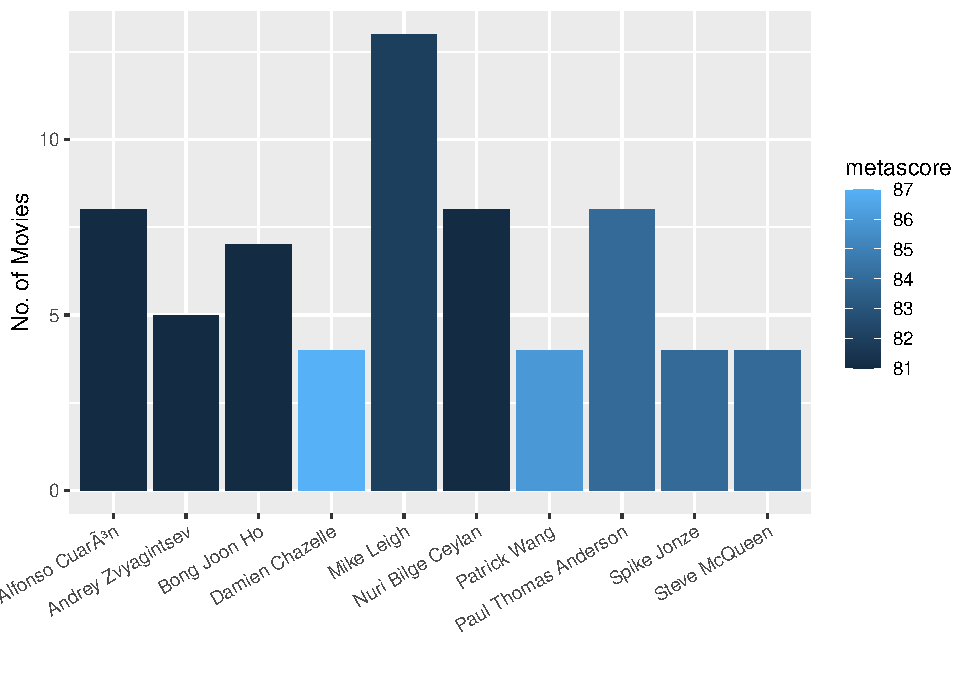
\includegraphics{Report_files/figure-latex/dirfig2-1.pdf}
\caption{\label{fig:dirfig2}Total number of movies for Top Directors}
\end{figure}

\hypertarget{top-grossing-movie}{%
\subsection{Top Grossing Movie}\label{top-grossing-movie}}

In this section, we'll look at the top grossing movie of the most successful directors that we established from Table \ref{tab:dirtab}.

\begin{table}[!h]

\caption{\label{tab:dirtab2}Director Top grossing movies}
\centering
\begin{tabular}[t]{l|l|l}
\hline
Director & Highest Grossing Movie & Total Revenue\\
\hline
\cellcolor{gray!6}{Alfonso Cuarón} & \cellcolor{gray!6}{Harry Potter and the Prisoner of Azkaban} & \cellcolor{gray!6}{\$796,093,802}\\
\hline
Damien Chazelle & La La Land & \$446,092,357\\
\hline
\cellcolor{gray!6}{Steve McQueen} & \cellcolor{gray!6}{12 Years a Slave} & \cellcolor{gray!6}{\$187,733,202}\\
\hline
Bong Joon Ho & Gisaengchung & \$109,012,467\\
\hline
\cellcolor{gray!6}{Spike Jonze} & \cellcolor{gray!6}{Where the Wild Things Are} & \cellcolor{gray!6}{\$100,086,793}\\
\hline
Paul Thomas Anderson & There Will Be Blood & \$76,181,545\\
\hline
\cellcolor{gray!6}{Mike Leigh} & \cellcolor{gray!6}{Mr. Turner} & \cellcolor{gray!6}{\$22,179,785}\\
\hline
Andrey Zvyagintsev & Vozvrashchenie & \$8,482,993\\
\hline
\cellcolor{gray!6}{Nuri Bilge Ceylan} & \cellcolor{gray!6}{Kis Uykusu} & \cellcolor{gray!6}{\$4,018,705}\\
\hline
Patrick Wang & In the Family & \$101,934\\
\hline
\end{tabular}
\end{table}

It can be observed from Table \ref{tab:dirtab2} that the \emph{Alfonso Cuarón} is the director of the top grossing movie \emph{Harry Potter and the Prisoner of Azkaban} which made \$796,093,802 worldwide. Followed by, \emph{Damien Chazelle}, the director of \emph{La La Land} grossing \$446,092,35. Suprisingly, \emph{Patrick Wang}, with an average metascore of 86 and a total of 4 movies made the least at just \$101,934.

\begin{figure}[H]

{\centering 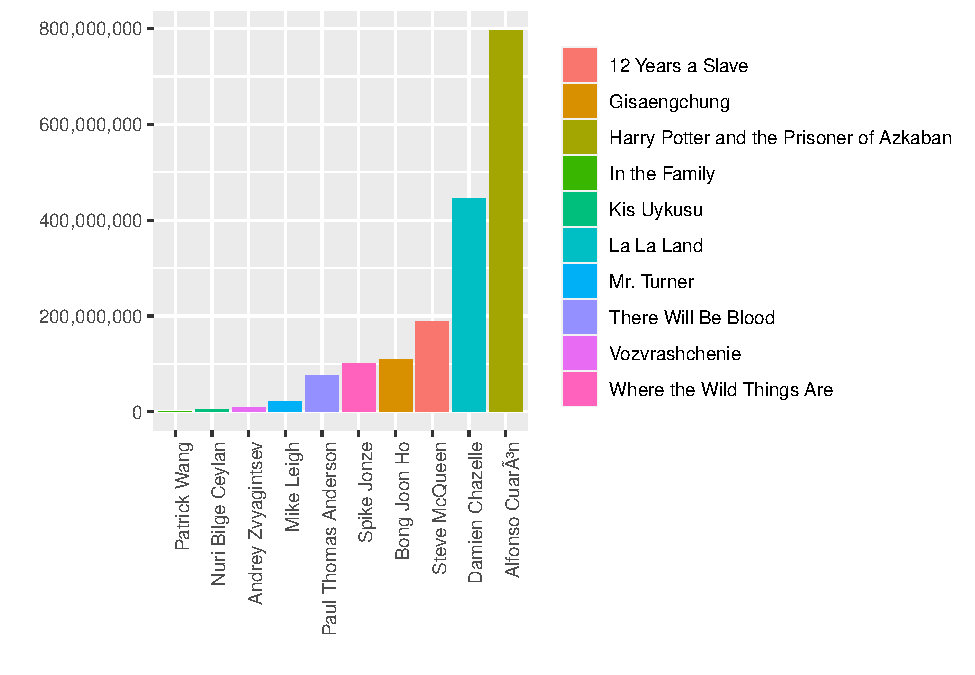
\includegraphics{Report_files/figure-latex/4-1} 

}

\caption{Top Grossing Movies}\label{fig:4}
\end{figure}

\hypertarget{movie-length-and-language-analysis}{%
\subsection{Movie Length and Language Analysis}\label{movie-length-and-language-analysis}}

\hypertarget{lets-look-at-some-of-the-common-movie-languages.}{%
\subsubsection{Let's look at some of the common movie languages.}\label{lets-look-at-some-of-the-common-movie-languages.}}

\begin{table}[!h]

\caption{\label{tab:langtab}Number of movies per language}
\centering
\begin{tabular}[t]{l|r}
\hline
Language & Number of Movies\\
\hline
\cellcolor{gray!6}{English} & \cellcolor{gray!6}{34519}\\
\hline
multi-lingual & 15188\\
\hline
\cellcolor{gray!6}{French} & \cellcolor{gray!6}{3777}\\
\hline
Spanish & 2640\\
\hline
\cellcolor{gray!6}{Japanese} & \cellcolor{gray!6}{2605}\\
\hline
Italian & 2565\\
\hline
\cellcolor{gray!6}{Hindi} & \cellcolor{gray!6}{1930}\\
\hline
German & 1702\\
\hline
\cellcolor{gray!6}{Russian} & \cellcolor{gray!6}{1235}\\
\hline
Turkish & 1229\\
\hline
\end{tabular}
\end{table}

From the Table \ref{tab:langtab}, it is quite clear that most movies are released in either only \emph{English} or in \emph{multi-lingual} format.

\hypertarget{is-there-a-pattern-in-movie-length-for-various-languages}{%
\subsubsection{Is there a pattern in Movie length for various languages?}\label{is-there-a-pattern-in-movie-length-for-various-languages}}

\begin{table}[!h]

\caption{\label{tab:langtab2}Average movie duration for all languages}
\centering
\begin{tabular}[t]{l|r}
\hline
Language & Avg. Movie Duration\\
\hline
\cellcolor{gray!6}{English} & \cellcolor{gray!6}{93.50190}\\
\hline
French & 99.38734\\
\hline
\cellcolor{gray!6}{German} & \cellcolor{gray!6}{96.43831}\\
\hline
Hindi & 140.40466\\
\hline
\cellcolor{gray!6}{Italian} & \cellcolor{gray!6}{98.94191}\\
\hline
Japanese & 102.96161\\
\hline
\cellcolor{gray!6}{multi-lingual} & \cellcolor{gray!6}{106.46787}\\
\hline
Russian & 99.78219\\
\hline
\cellcolor{gray!6}{Spanish} & \cellcolor{gray!6}{97.35833}\\
\hline
Turkish & 96.79170\\
\hline
\end{tabular}
\end{table}

\begin{figure}[H]

{\centering 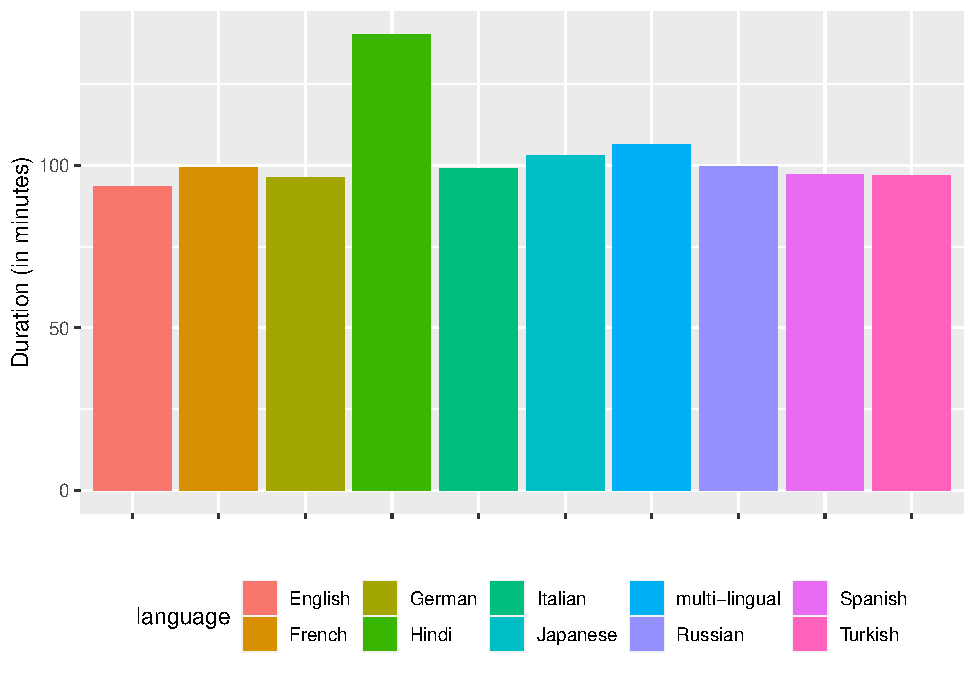
\includegraphics{Report_files/figure-latex/langfig-1} 

}

\caption{Movie Duration for different Languages}\label{fig:langfig}
\end{figure}

From the Figure \ref{fig:langfig}, we can infer that \emph{Hindi} movies are usually much longer than other languages clocking at an average runtime of 140 minutes. While, \emph{English} movies are usually the shortest at just 93 minutes.

\hypertarget{conclusion}{%
\section{Conclusion}\label{conclusion}}

\textbf{William's Section Conclusion}

There appears to be a strong correlation between movies that have been given extremely high ratings and the mid 1950's. However, due to the inherent bias within this data set, it is still impossible to identify which periods truly experienced a higher quality of movie production.

\textbf{Xue's Section Conclusion}

In conclusion, the English movie has the largest proportion of language movies within ten years, the drama movie is the favorite movie in all the country.

\textbf{Rahul's Section Conclusion}

In conclusion, we can see a general trend that a movie that is most talked about by the users or fans has grossed the most amount of money compared to lesser popular movies. The number of reviews by users can generally be used to predict if it was a box office hit.

\textbf{Aryan's Section Conclusion}

For Director analysis, it is clear from Figure 1 and Figure 2 that there is no one single way to measure success and that all directors in the list are doing very good in their own ways.

And from the Movie length analysis, we can infer that Hindi Movies are usually significantly longer than any other kind of movies. Also, english movies are among the shortest. We also concluded that movie language has an impact on movie length.

\hypertarget{citations}{%
\section{Citations}\label{citations}}

tidyverse \textcite{tidyverse}

dplyr \textcite{dplyr}

kableExtra \textcite{kableExtra}

treemap \textcite{treemap}

viridis \textcite{viridis}

scales \textcite{scales}

\printbibliography

\end{document}
